\section{Foundations}
\subsection{Derivation of EOM of many body system}
Hamiltonian of single atom dispersively coupled to single cavity mode by a running-wave laser drive 
\begin{equation}
	\hat{H}_{SP} = \frac{\hat{p}^2}{2M}- \hbar \omega_z \hat{F}_z + \hbar q \hat{F}^2_z + \hbar \omega_c \hat{a}^\dag \hat{a}-i \frac{\alpha_\nu}{2F}\left [ \bm{\hat{E}}^{(+)} \cross \bm{\hat{E}}^{(-)} \right ] \cdot \bm{\hat{F}} .
\end{equation}
Operator $\hat{a}$ creates photon in z-polarized cavity mode of frequency $\omega_c$. Second and third term are Zeeman splittings. $\bm{\hat{F}}$ is spin operator.
\begin{figure}[h!]
	\centering
	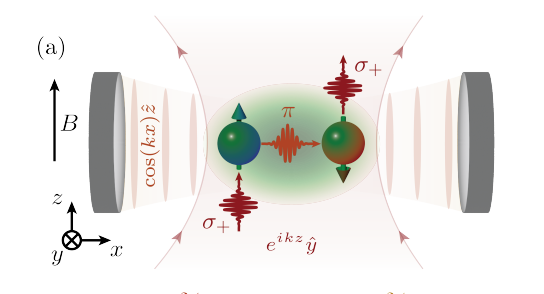
\includegraphics[width=1\linewidth]{Images/scetch_pair_production.png}
	\caption{Pair production}
	\label{fig:scetch_pair_production}
\end{figure}
\\ \break
Second quantization 
\\ \break
Spinor field operator \text{RHS "5-mode-expansion" doesnt contain second summand}
\begin{equation}
	\hat{\Psi} (\bm{x}) = \left (
	\begin{matrix}
		\frac{k}{\sqrt{2}\pi} \cos(kx) ( e^{ikz}\hat{c}_{+k,+1} + e^{-ikz} \hat{c}_{-k,+1})
		\\
		\frac{k}{2 \pi}\hat{c}_{0,0} + \frac{\sqrt{2}k}{\sqrt{3}\pi} \cos^2(kx)\hat{c}_{\pm2k_x,0}
		\\
		\frac{k}{\sqrt{2}\pi} \cos(kx) ( e^{-ikz}\hat{c}_{-k,-1} + e^{ikz} \hat{c}_{+k,-1})
	\end{matrix} \right)
	= \left (
	\begin{matrix}
		\hat{c}_{+1,+k} \psi_{+1,+k} + \hat{c}_{+1,-k} \psi_{+1,-k}
		\\
		\hat{c}_{0,0}\psi_{0,0} 
		\\
		\hat{c}_{-1,k} \psi_{-1,+k} + \hat{c}_{-1,-k}\psi_{-1,-k}
	\end{matrix}
	\right)
\end{equation}
Where the respective functions have to be normed
\begin{equation}
	\int_{\frac{-\pi}{k}}^{\frac{\pi}{k}}  \psi^*_{+1,+k} \psi_{+1,+k} dz dx = 1
\end{equation}(c.f. 2010 Dicke paper)
\begin{equation}
	\Psi = \left( \begin{matrix}
		\Psi_{+1}
		\\
		\Psi_0
		\\
		\Psi_{-1}
	\end{matrix}\right)
\end{equation}
Next we find an effective many body hamiltonian.
\begin{equation}
	H_{SP} = H_L + H_{AT} + H_{INT}
\end{equation}
Where $H_{AT}$ contains $F_z$ and $H_{INT}$ contains $F_+, F_-$.
\begin{equation}
	H_{MB} = H_L + \int \hat{\Psi}^\dag(\hat{x}) ( H_{AT} + H_{INT}) \hat{\Psi}(\hat{x}) \hat{dx}
\end{equation}

e.g. 
\begin{equation}
	F_z = \left( 
	\begin{matrix}
		+1 && 0 && 0
		\\
		0 && 0 && 0 
		\\ 
		0 && 0 && -1
	\end{matrix}
	\right) 
\end{equation}
\begin{equation}
	F_+ =\sqrt{2} \left( 
	\begin{matrix}
		0 && 1 && 0
		\\
		0 && 0 && 1 
		\\ 
		0 && 0 && 0
	\end{matrix}
	\right) 
\end{equation}
This calculation is done in Rodrigos "Full derivation Hamiltonian" handwritten pdf. We do adiabatic elimination with effective operators and apply the rotating wave approximation. 
We obtain the effective many-body Hamiltonian
\begin{equation}\label{eq:fou_effective_many_body_hamiltonian}
	H = H_0 + H_+ + H_-
\end{equation}
with e.g.
\begin{equation}
	H_+ = \hbar \chi_+ (2 \hat{c}^\dag_{-k,-1} \hat{c}^\dag_{+k,+1}\hat{c}_0 \hat{c}_0+ \hat{c}^\dag_0 \hat{c}_{+k,+1}\hat{c}^\dag_{+k,+1}\hat{c}_0 + \hat{c}^\dag_{-k,-1}\hat{c}_0\hat{c}_0^\dag \hat{c}_{-k,-1} + h.c.)
\end{equation}
\subsection{Further info to experiment: (rodrigo thesis p.103)}
drive is operated in limit of large two-poton  detunings
\begin{equation}
	|\delta_\pm| \gg \kappa
\end{equation}
\begin{equation}
	\delta_\pm = \delta_c \pm \omega_z = (\omega_d \pm \omega_z) - \omega_c
\end{equation}
We absorb drive photon, and go from 
\begin{equation}
	\ket{0}_0 \rightarrow \ket{+k}_+1
\end{equation}
thus we need a energy conserving cavity photon with freq $\approx \omega_d - \omega_z$. (or $+\omega_z$?) Here we can still ignore the kinetic energy $\sim k$ of the atom since this energy is much smaller than $\kappa$.
\\ 
Parametric amplification of pair production
\\
look at \ref{eq:fou_effective_many_body_hamiltonian} + assume mode $\ket{0}_0$ undepleted throughout the dynamics i.e. occupied by N atoms. set $\hat{c}_0$ = $\sqrt{N}$ and obtain
\begin{equation}
	\hat{H}_{eff} = \hat{H}^+_{eff} + \hat{H}^-_{eff}
\end{equation}
with 
\begin{equation}
	\hat{H}^\pm_{eff} = \hbar (\omega_0 + 4 N \chi_\pm)(\hat{K}_{z,\pm}-1/2) + 4 \hbar N \chi_\pm \hat{K}_{x,\pm}
\end{equation}
Look at linear equations of motion
\begin{equation}\label{eq:fou_time_development_linear_K}
	\dt{}\left( 
	\begin{matrix}
		\hat{K}_{x,\pm}
		\\
		....y
		\\
		...z
	\end{matrix}\right) = \bm{M}_\pm 
	\left( \begin{matrix}
	\hat{K}_{x,\pm}
	\\
	....y
	\\
	...z
	\end{matrix}\right)	
\end{equation}
with three non-degenerate complex eigenvalues
\begin{align}
	\lambda_{1,\pm} = 0 
	\\
	\lambda_{2,\pm} = \sqrt{-\omega_0(\omega_0 + 8 N \chi_\pm)} \eqcolon + \lambda_\pm
	\\
	\lambda_{3,\pm} = - \sqrt{- \omega_0 (\omega_0+8N \chi_\pm)}
\end{align}
We also have

\begin{equation}\label{eq:fou_time_development_particle_number}
	\langle N_{p,\pm} \rangle = \frac{1}{2} (\langle c_{1,\pm}^\dag c_{1,\pm} \rangle + \langle c_{-1,\mp}^\dag c_{-1,\mp}\rangle ) \approx \langle K_{z,\pm} \rangle - \frac{1}{2} \approx A\cosh(\lambda_\pm t) + \text(const)
\end{equation}
To conclude: we see that we have eigenvectors of M. Those are perpendicular, since the eigenvalues are different. The time development of those is given by \ref{eq:fou_time_development_linear_K}. Thus, its either phase oszillation for a complex eigenvalue or exponential growth for a real eigenvalue. \ref{eq:fou_time_development_particle_number} looks at the expectation value of the occupation of the modes that are not $\ket{0}_0$ (occupation of pairs). we see that the time development of those depends on $ \langle K_{z,\pm} \rangle$, therefore on the eigenvectors of M, therefore on the eigenvalues of M. We see, that for a real $\lambda_\pm$ the occuopation of those modes get macroscopic. So we say that for a critical coupling a second order phase transition occurs (lambda get real) featuring pairs. this fast change of coupling is called quench (faster that any period of oscillations happening in system e.g. $1/\omega_0$). 
\\
Note: if the number of pairs gets high, the undepleted approximation doesnt hold anymore. thus this equations can just predict the inital growth of pairs. (later there is saturation)
\\
quench: the system jumps from one set of eigenstates to another set of eigenstates. before system was in single eigenstate, after quench it is superposition of different eigenstates $\rightarrow$ oscillation of those. this cant be expressed analytically, thus calculations are done numerically. 
\begin{figure}[h!]
	\centering
	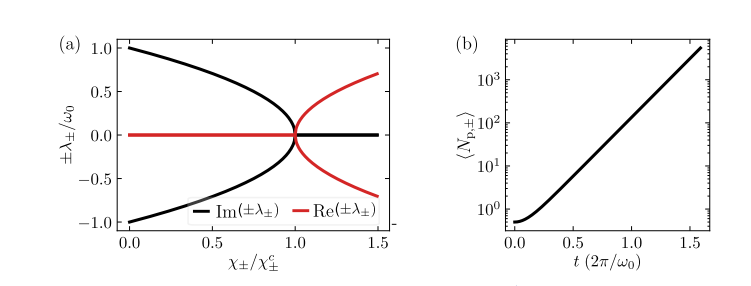
\includegraphics[width=1\linewidth]{Images/scetch_quench_parametric_amplification.png}
	\caption{Parametric amplification}
	\label{fig:scetch_quench_parametric_amplification}
\end{figure}
\subsection{The energy scales}
not sure, whether all plus /minus are choosen correctly in scetch, but the scheme looks approximately like this:  
\begin{figure}[h!]
	\centering
	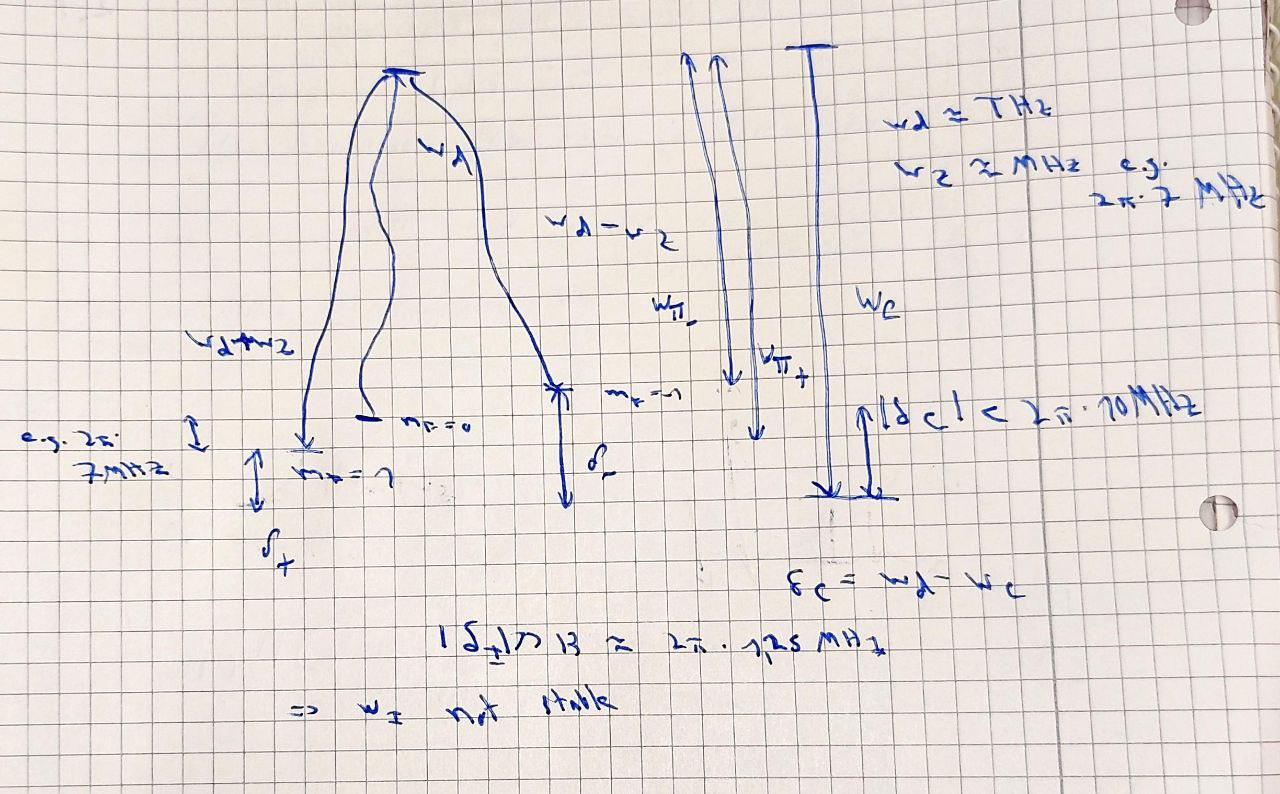
\includegraphics[width=1\linewidth]{Images/energy_scetch.jpeg}
	\caption{Energy scetch}
	\label{fig:energy_scales}
\end{figure}
We start in the Rb87 5 2 S1/2 F=1 (F... total angular momentum) fine structure) (https://steck.us/alkalidata/rubidium87numbers.1.6.pdf). We send light $\omega_d$ with $\lambda 790.02nm$. The transition to the  5 2 P3/2 (D2 transition) is around 980nm the transition to 5 2 Pb1/2 (D1) is around 995nm. thus, we are blue detuned with D1 and red detuned with D2 (check whether its not other way around)(one of the wavelength in Rb is wrong). This is called Tune out-wavelength. Even though it is not exactly the middle it is the effective middle. So the scalar polarization $\alpha_s$ is zero and there is no dipole potential trapping the atom. We are off resonant by THz and therefore wont reach any population in the 5 2 P levels (dispersive regime). N I S H A N T  Dogra phdthesis ch3.1. explains this detailed. 
\\
the energy of the $\pi$ photon is $\omega_\pm$ = $\omega_d \pm w_z$. So something like Thz $\pm$ e.g. $\omega_z = 2\pi 7 $MHz.
\\
The cavity wavelength is chosen to be similar to the drive wavelength: $|\delta_c| = |\omega_d - \omega_c| < 2\pi 10$MHz. But the cavity wavelength is off resonant to the $\pi$ photon wavelength if we compare this detuning $\delta_\pm$ (= diff $\omega_\pm$ and $\omega_c$) with the cavity loss $\kappa$. $|\delta_\pm | \gg \kappa$
\\
From somewhere we get
\begin{equation}\label{eq:fou_coupling}
	\chi_\pm = \eta^2 \frac{\delta_\pm}{\delta_\pm^2 + \kappa^2}
\end{equation}
and
\begin{equation}
	\gamma_\pm = \frac{\eta^2 \kappa}{\delta_\pm^2 + \kappa^2}.
\end{equation}
\begin{equation}
	\eta \sim \alpha_\nu E_d E_0
\end{equation}
where $\alpha_\nu$ vectorial polarisierbarkeit, $E_d$ amplitude of drive, $E_0$ electric field of vacuum of cavity mode =$\rangle$ given by geometry.
\\
concrete we have
\begin{equation}
	\eta = \beta \alpha_\nu E_0 E_d / 8 \hbar.
\end{equation}
The factor $\beta \approx 0.89$ arises from overlap integrals between harmonically confined atomic cloud, the cavity mode and the drive.
\\
 (\ref{eq:fou_coupling}) shows, that for high $\omega_z$ the first atom will be most likely in state $\ket{+k,+1}$. This is because high $\omega_z$ implies high $| \delta_- |$ and small $| \delta_+ |$ which leads to a stronger coupling for the + channel. 
\\
Experimentally we can change $\delta_c$ and $\omega_z$.  
\\ 
 how is k defined? $k=k_z$?. own consideration: let $\omega_c$ = $\omega_d$ + x, where x is order of MHz. We get by Taylor
 \begin{equation}
 	\lambda_c = \frac{c}{\omega_d + x} = \frac{c}{\omega_d}- x \frac{c}{\omega_d^2} + O(x^2) \approx \frac{c}{\omega_d} = \lambda_d.
 \end{equation}
Thats the reason, why we use for python just one single wavelength $\lambda_M$. So we can conclude that $k_z \approx k_x$ (=k, right?). 
 \\
 With this result we look at the energies of different states: 
 \begin{equation}
 	\psi_{\pm 2 k, 0} \approx N \cos(2kx) \otimes \ket{m=0}
 \end{equation}
 and therefore
 \begin{equation}
 	E_{rec} = \frac{\hbar^2 (2k)^2}{2m} = \hbar 4 \omega_{rec}
 \end{equation}
 with 
 \begin{equation}
 	\omega_{rec} =  \frac{\hbar k^2}{2m}
 \end{equation}
 (check formulas, rodrigo gave them to me.).
 \\
 We also get
 \begin{equation}
 	\psi_{+k,+1} \approx N \cos(kx)e^{ikz}.
 \end{equation}
\begin{align}
	E_{kin} &= \int \psi_{+k,+1} \hbar \left ( \frac{\partial_x^2 + \partial_y^2}{2m} \right) \psi_{+k,+1} dx dz
	\\
	& =\frac{\hbar k_x^2 + \hbar k_z^2}{2m} = 2 \omega_{rec}.
\end{align}
So if we consider the creation of a single pair, we get that this pair has energy 
\begin{equation}
	\omega_0 = 2q + 4 \omega_{rec}
\end{equation} 
in comparison to the to atoms in the BEC. The first order zeeman splitting cancelled out such that only the 2nd order Zeeman splitting q and the kinetic energy $\omega_{rec}$ contribute. (check with rodrigo, whether this is correct understanding. for this understanding we dont need to consider rotating frame.). We see that for small q the $\ket{\pm 2k,0}$ and $\ket{+k,+1}$ modes have the same energy scale. 
\\
Derivation of recoil energy:
\begin{equation}
	E_{rec} = \frac{p_{rec}^2}{2m} = \frac{\hbar^2 k^2}{2m} = \frac{\hbar^2 4 \pi^2}{2 m \lambda^2} = \hbar \omega_{rec}.
\end{equation}
\subsection{Number squeezing}
Following (thesis Finger)
\\
Introduce imbalance operator
\begin{equation}
	\hat{J}_z = \frac{1}{2} (\hat{N}_{+1}- \hat{N}_{-1})
\end{equation}
where $\hat{N}_{+1} = \hat{c}_{+k,+1}^\dag \hat{c}_{+k,+1}$ and $\hat{N}_{-1} = \hat{c}_{-k,-1}^\dag \hat{c}_{-k,-1}$. 
We introduce 
\begin{equation}
	\xi_N^2 = \frac{4 \sigma^2(\hat{J}_z)}{N}
\end{equation}
where $\sigma^2(\hat{J}_z)$ is variance of imbalance operator. Normalize to the squeezing parameter $\xi_{N,coh}^2$ of uncorrelated spin coherent state $\sigma^2(\hat{J}_z) = \langle N_p \rangle / 2$. If the expression
\begin{equation}
	\frac{\xi_N^2}{\xi^2_{N,coh}} = \frac{2 \sigma^2(\hat{J}_z)}{\langle N_p \rangle}
\end{equation} 
gets smaller than one, the N-atom state is squeezed below the standard quantum limit. (i.e. below the fluctuations associated with a coherent spin state). 
\\
We choose sound initial values:N = 80000,eta = 2*np.pi*1.7e3 ,Kappa = 2*np.pi*1.25e6, omegaZ = 2*np.pi *7.09e6,deltaC = -2*np.pi *25.8e6 and get deltap = -117558397.09733006 and xp=(eta**2*deltap/(deltap**2+(Kappa)**2))/1000 , Pair coupling for chi+ Channel: xp =-0.0009662. In the following we hold this coupling constant.

\subsection{Bipartie entanglement} (following finger thesis)

Assume small Zeeman splittings $\omega_z \rightarrow 0$ (which means two-channel configuration) , where both couplings $\mu_+ \approx \mu_- = \mu$ become equal (what is difference between $\mu$ and $\chi$?). We get
\begin{equation}
	\ket{\psi} = (1-\mu^2) \sum_{N_p^+,N_p^- = 0}^\infty \mu^{N_p^+ + N_p^-} \ket{N_p^+,N_p^+;N_p^-.N_p^-}
\end{equation}
Thus, for high-gain limit $\mu \rightarrow 1$ our state consists of a superposition of many pair states with different pair numbers. State is called 'entangled bright squeezed vacuum state'
\\
signal atoms go in +z direction(A), idler atoms in -z direction(B). Thus, we can see this as two subsystems A, B. Introduce collective pseudo-spin operator: 
\begin{equation}
	\bm{J}_{A,B} = \sum_n^{N_{A,B}} \bm{j}_n 
\end{equation}
fullfilling
\begin{equation}
	\bm{J} = \bm{J}_A+ \bm{J}_B
\end{equation}

\subsection{Spin-nematic squeezing} (following kunkel thesis)https://www.kip.uni-heidelberg.de/Veroeffentlichungen/download.php/6440/temp/3991.pdf
Spin-1 states: we have basis $\ket{m_F}$ with $m_F \in \{-1,0,+1\}$ for the F = 1 hyperfine manifold
\\ 
Pure $\textbf{single-particle}$ state is (up to a global phase)
\begin{align}
	\ket{\psi} &= r_{+1} e^{i \Phi_L /2} \ket{+1} + r_0 e^{i\Phi_S} \ket{0} + r_{-1} e^{-i \Phi_L /2} \ket{-1}
	\\
	& = \left (
	\begin{matrix}
		r_{+1}e^{i \Phi_L/2}
		\\
		r_0 e^{i\Phi_S}
		\\
		r_{-1} e^{i \Phi_L/2}
	\end{matrix} \right )
\end{align}
where prefactors $r_{0,\pm 1}$ are chosen real with $\sum_i r_i^2 = 1$. 
\\
Lamor phase defined
\begin{equation}
	\Phi_L = \Phi_{+1}- \Phi_{-1}
\end{equation}
Spinor phase defined (sometimes differs in literature)
\begin{equation}
	\Phi_S = \Phi_0 - ( \Phi_{+1} - \Phi_{-1})
\end{equation}
Aim to find complete set of operators which form a basis for hermitian operators acting on spin-1 Hilbert space to completely describe the density matrix of a mixed state. 
\begin{equation}
	\hat{\bm{S}}_x = \frac{1}{\sqrt{2}}\left( 
		\begin{matrix}
				0 && 1 && 0
				\\
				1 && 0 && 1
				\\
				0 && 1 && 0
		\end{matrix} \right)
\end{equation}
they (as sigma matrices in spin 1/2 case) fulfill SU(2) commutation relation $[\hat{\bm{S}}_i,\hat{\bm{S}}_j] =i \epsilon_{ijk} \hat{\bm{S}}_k$. In contrast to spin-1/2 case, mean value of these three operators are not sufficient to uniquely determine the quantum state. eg in thesis. thus, additional observables required to unambiguously identify the spin states.
//
Here: quadrupole operators
\begin{equation}
	\hat{\bm{Q}}_{ij} = \hat{\bm{S}}_i \hat{\bm{S}}_j + \hat{\bm{S}}_j \hat{\bm{S}}_i - \frac{4}{3} \delta_{ij} \mathds{1}_3
\end{equation}
Together with spin operators this gives 9 operators. 
\\
own thoughts: spin1/2: pure state: 2 free components, mixed state three free components $\rightarrow$ $\vec{r}$ to define (so density matrix has 3 independent entries. this goes also along with the picture of a 2x2 matrix., wait, but the entries of the density matrix are complex, this would double the amount of free components. i dont get it.). spin 1: pure state 4 free components (two real parts + two complex phases). 
//
Density matrix has 8 independent entries. (this goes along with the picture of a 3x3 matrix, but wait. complex entries, so this time complex 8D hilbert space over complex field?). Thus, basis set is overcomplete. We only choose the following five quadrupole operator:
\begin{equation}
	\xo{Q}_{xz} = \frac{1}{\sqrt{2}} \left (
	\begin{matrix}
		0 && 1 && 0 
		\\
		1 && 0 && -1
		\\
		0 && -1 && 0
	\end{matrix} \right ), \xo{V}_x = \frac{1}{2} (\xo{Q}_{xx} - \xo{Q}_{yy}) = \left( 
	\begin{matrix}
		0 && 0 && 1
		\\
		0 && 0 && 0
		\\
		1 && 0 && 0
	\end{matrix} \right)
\end{equation}etc.
With these operators a general spin-1 density matrix is parametrized as
\begin{equation}
	\hat{\rho} = \frac{1}{3} \mathds{1}_3 + \sum_i s_i \xo{S}_i  + \sum_j q_j \xo{Q}_j + \sum_k v_k \xo{V}_k
\end{equation}.
Quadrupol operators are linked to second moment of the spin i.e. the covariance matrix
\begin{align}
	T_{ij} &\coloneqq \frac{1}{2} \langle \xo{S}_j \xo{S}_i + \xo{S}_i \xo{S}_j \rangle_Q - \langle \xo{S}_i \rangle_Q \langle \xo{S}_j \rangle_Q
	\\ 
	&= \langle \frac{1}{2} \xo{Q}_{ij} + \frac{1}{3} \delta_{ij}  \mathds{1}_3 \rangle_Q - \langle \xo{S}_i \rangle_Q \langle \xo{S}_j \rangle_Q
\end{align}
where $\langle .  \rangle_Q $ is quantum mechanical expectation value $tr\{\cdot \rho \}$.
\\
The density matrix of a general single-particle mixed state is, thus, defined by mean value of there eight operator. (mean value of those operators: eg $\xo{S}_i$: mean value is $ \langle\xo{S}_i \rangle = Tr\{ \rho \xo{S}_i \}$. Let us add inner product to Hilberspace(wait the operator space is just a vector space, right? a hilbertspace would already have an inner product), let this be defined for A,B as $Tr\{ AB\}$: then we only have to check, that our operators are orthonormal under this inner product (and with Id?). If yes, we get that the prefactors are given by the mean value of the corresponding operator (as stated before)).
\\
We have the SU(2) subspaces $\{\xo{S}_x, \xo{S}_y, \xo{S}_z\}, \{\xo{Q}_{xz},\xo{Q}_{yz}, \xo{S}_z\}, \{\xo{V}_x, \xo{V}_y, \xo{S}_z\}.$. Notice: all three subspaces contain operator $\xo{S}_z$ and rotation around corresponding axis is equivalent to change of Larmor phase. Thus, in a Hesinberg picture the remaining two operatros in each SU(2) subspace are connected via a change of the Lamor phase. 
\\
Transversal operators
\begin{align}
	\xo{S}_\perp (\Phi_L) \coloneqq \cos(\Phi_L) \xo{S}_x + \sin(\Phi_L) \xo{S}_y
	\\
	...
	\\
	\xo{V}_\perp (\Phi_L) \coloneqq \cos(2\Phi_L) \xo{V}_x + \sin(2\Phi_L) \xo{V}_y
\end{align}
\\
Similar $\xo{Q}_{zz}$ is connected to spinor phase $\Phi_S$. We want to represent the unitary operation $e^{-i \varphi \xo{Q}_{zz}/2}$ on some SU(2) sphere where the rotations are generated by $\xo{Q}_{zz}$. Define 
\begin{equation}
	\xo{Q}_0 \coloneqq - \frac{1}{3} \mathds{1}_3 - \xo{Q}_{zz} = \left(
	\begin{matrix}
		-1 && 0 && 0 
		\\
		0 && 1 && 0 
		\\ 
		0 && 0 && -1
	\end{matrix}
	\right)
\end{equation} 
to center the spectrum around zero. 
\\
With this operator we define the spin-nematic subspace $\{\xo{S}_\perp(\Phi_L), \xo{Q}_\perp(\Phi_L), \xo{Q}_0\}$ for each phase $\Phi_L$. ... In general they do not fulfill the SU(2) commutation relations. However for states $\ket{\psi_n}$ with equal probability to find a particle in the state $\ket{\pm 1}$ one can find a phase $\Phi_L$  with $\langle \xo{N}^+ - \xo{V}_\perp(\Phi_L)\rangle_Q = 0$. The operators then fulfill the SU(2) permutation relations for the expectation value
\begin{equation}
	\langle [ \xo{Q}_\perp (\Phi_L), \xo{S}_\perp (\Phi_L) ] \rangle_Q = 2 i \langle \xo{Q}_0 \rangle_Q.
\end{equation}
Discussion Rodrigo: we define it that general with Q,Sperp, because we can decide on the lamour phase and therefore it can be either Sx or Sy or sth in between.
\\
This commutation relation means that they have this SU(2) rotation relation.e.g. rotating around $Q_0$ axis rotates a state in $S_\perp$ to a state in $Q_\perp$ and vv. Not so sure but i think: The phase that creates the roations with the generator $Q_0$ is the spinor phase. Maybe $\exp{-i \Phi_S \xo{Q}_0}$. well, in the figure it is $Q_{yz}, S_x$. so $S_\perp$ and $Q_\perp$ are connected by Spinor phase.
\\
Any unitary trafo generated by these three operators does not change $\Phi_L$.
\\
done with chapter!
\\
now following chapman paper: spin-nematic squeezed vacuum in a quantum gas
\\
here: look at multi particle formalism.
\\
We define
\begin{equation}
	\hat{S}_x = \frac{1}{\sqrt{2}}( \hat{a}_1^\dag \hat{a}_0 + \hat{a}_0^\dag \hat{a}_{-1} + \hat{a}_0^\dag \hat{a}_1 + \hat{a}_{-1}^\dag \hat{a}_0)
\end{equation}
Generalized uncertainty relation
\begin{equation}
	\Delta A \Delta B \geq \frac{1}{2} |\langle [A,B] \rangle |
\end{equation}
E.g. all atoms in $m_f = 0$. We get 
\begin{equation}
	\bra{0,N,0} [\hat{S}_x , \hat{Q}_{yz} ] \ket{0,N,0} = - 2iN
\end{equation}
Relevant uncertainty relation
\begin{equation}
	\Delta S_x \Delta Q_{yz} \geq N
\end{equation}
Define squeezing parameter (in terms of quadratures of the operators: which operators? I guess Sx and Qyz, because cos theta Sx + sin theta Qxy =: quadrature operator)
\begin{equation}
	\xi_{x}^2 = \langle ( \Delta (\cos \theta S_{x} + \sin \theta Q_{yz}))^2 \rangle /N
\end{equation}
with $\theta$ as the quadrature angle. Squeezing if variance of quadrature operator being less than SQL of N for some value of $\theta$. 
Therefore if $\xi_x^2 < 1$.
\\
protocol: Initial state $m_f = 0$. b) 25ms of evolution: spin nematic squeezing develops. c ) microwave pulse rotates quadrature phase around Qzz. Looking at kunkel thesis, this could be the spinor phase.  d) pi/2 RF pulse rotates transverse magnetization Sx into Sz (so rotation around Sy?).e) we now measure Sz thus before in c) Sx was squeezed. And before that in b) an arbitrary quadrature of cos theta Sx + sin theta Qyz was squeezed. 
\\
So which states to we need to squeeze this quadrature operator? Do we have them in our experiment? Which quadrature is squeezed? Do we have the pulses experimentally to rotate the squeezing it in the Sz direction?
\begin{figure}
	\centering
	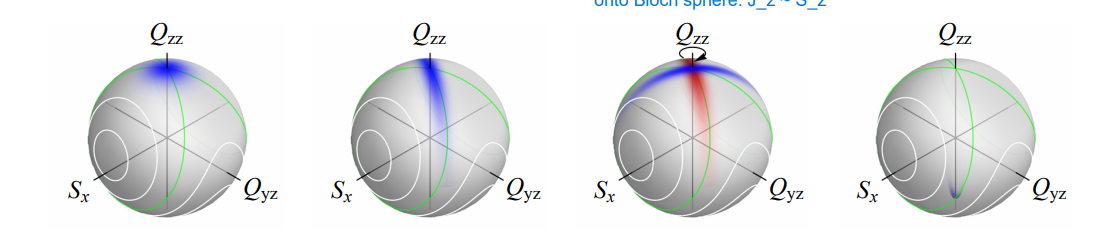
\includegraphics[width=0.7\linewidth]{chapman_fig1}
	\caption{}
	\label{fig:chapmanfig1}
\end{figure}










 


